\documentclass{article}

\usepackage{fontspec}
\usepackage{polyglossia}
\usepackage{notomath}
\setmainfont{GFS Artemisia}
\setsansfont{Source Code Pro}
\setmonofont{Source Code Pro}
\newfontfamily\greekfont[Script=Greek]{GFS Artemisia}
\newfontfamily\greekfontsf[Script=Greek]{GFS Artemisia}
\newfontfamily\greekfonttt[Script=Greek]{Source Code Pro}

%languages
\setdefaultlanguage{greek}
\setotherlanguages{english}


%typing
\usepackage{hyphenat}
\usepackage{float}
\usepackage{color, colortbl}
\usepackage{placeins}

%captions
\usepackage{caption}
\usepackage{subcaption}

%bib
% \usepackage{biblatex}
% \addbibresource{bib.bib}

%gemoetry
\usepackage[a4paper,top=1.2cm,bottom=1.2cm,left=1.2cm,right=1.2cm,marginparwidth=1.5cm]{geometry}

%images
\usepackage{graphicx}
\usepackage{tikz}

%ref
\usepackage[colorlinks=true, allcolors=blue]{hyperref}


\usepackage[export]{adjustbox}

%label
\usepackage{enumitem}
\renewcommand{\labelenumii}{\arabic{enumi}.\arabic{enumii}}
\renewcommand{\labelenumiii}{\arabic{enumi}.\arabic{enumii}.\arabic{enumiii}}
\renewcommand{\labelenumiv}{\arabic{enumi}.\arabic{enumii}.\arabic{enumiii}.\arabic{enumiv}}

%columnnew
\newcolumntype{g}{>{\columncolor{gray}}l}

%colors
\usepackage[dvipsnames]{xcolor}
\definecolor{gray}{gray}{0.9}
\definecolor{blue}{RGB}{82, 138, 174}
\definecolor{green}{RGB}{140, 219, 169}
\definecolor{yellow}{RGB}{253, 221, 92}

% \usepackage{titling}
% \setlength{\droptitle}{-20em}             %allagh glwssas
\hypersetup{
    colorlinks = true,
    linkcolor=black}


\usepackage{autobreak}


%Customize tables
\renewcommand{\arraystretch}{1.2}
% \rowcolors{2}{gray}{white}



\captionsetup[table]{
    format=plain,
    labelfont={small,it,bf}, % Small, italic, and bold label
    textfont={small,it}, % Italic text
    labelsep=colon % Colon separator
}



% Customize the figure caption
\captionsetup[figure]{
    format=plain,
    labelfont={small,it,bf}, % Small, italic, and bold label
    textfont={small,it}, % Italic text
    labelsep=colon % Colon separator
}

\makeatletter
\renewcommand*{\p@table}{\textit{Πίν. }}
\renewcommand*{\p@figure}{\textit{Σχ. }}
\renewcommand*{\p@equation}{\textit{Εξ. }}
\makeatother


\begin{document}

%TITLE
\newcommand{\uni}{ΑΡΙΣΤΟΤΕΛΕΙΟ ΠΑΝΕΠΙΣΤΗΜΙΟ ΘΕΣΣΑΛΟΝΙΚΗΣ}
\newcommand{\faculty}{ΠΟΛΥΤΕΧΝΙΚΗ ΣΧΟΛΗ}
\newcommand{\tmhma}{ΤΜΗΜΑ ΜΗΧΑΝΟΛΟΓΩΝ ΜΗΧΑΝΙΚΩΝ}


\newcommand{\titlos}{Δυναμικά φαινόμενα}
\newcommand{\ypotitlos}{Bonus Εργασία - Ειδικά Κεφάλαια Πεπερασμένων Στοιχείων}


\newcommand{\onomaauthor}{ΒΑΣΙΛΕΙΟΣ ΠΑΠΑΜΙΧΑΗΛ}


\newcommand{\advisor}{Γάκιας Χρήστος}
\newcommand{\mailauthor}{\href{mailto:vasilepi@meng.auth.gr}{vasilepi@meng.auth.gr}}
\newcommand{\aem}{6920}
\newcommand{\hmeromhnia}{\today}



\begin{titlepage}
    \begin{center}
    \raisebox{20mm}{
    \begin{tikzpicture}
        \draw (0,0) -- (6,0);
    \end{tikzpicture}}
\includegraphics[width=4cm]{media/autheng.jpg}\raisebox{20mm}{\begin{tikzpicture}
        \draw (0,0) -- (6,0);
    \end{tikzpicture}}
     \end{center}
    
    \begin{center}
        \large
        \uni\\
        \normalsize
        \faculty\\
        \vspace{1em}
        \tmhma
    \end{center}

    \vspace{2cm}
    \begin{center}
        \Large
        \textbf{\titlos}\\
        \vspace{1em}
        \large
        \textit{\ypotitlos}
    \end{center}
    \begin{center}
        \begin{tikzpicture}
        \draw (0,0) -- (4,0);
    \end{tikzpicture}\\
    \vspace{7em}
    \Large
    \textcolor{BrickRed}{\textbf{\onomaauthor}}\\
    \vspace{3em}
    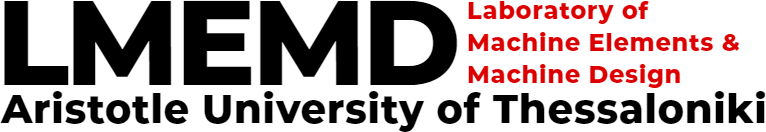
\includegraphics[width=0.3\textwidth]{media/newlogov3-cropped-content.png}
    \end{center}

    \vspace{7em}
    \hspace{4ex}
    \begin{minipage}[t]{0.45\textwidth} 
        \raggedright
        \textbf{Υπεύθυνος}: \advisor\\
        \textbf{Email}: \mailauthor\\
        \textbf{ΑΕΜ}: \aem
    \end{minipage}\\

    \vspace{4cm}
    \begin{center}
        \textit{\hmeromhnia}\\
        \begin{tikzpicture}
            \draw (0,0) -- (15,0);
        \end{tikzpicture}
    \end{center}
    
    
\end{titlepage}

\tableofcontents


\section{Εισαγωγή}
\subsection{Παρουσίαση προβλήματος}
Σκοπός της παρόν εργασίας είναι η επίλυση προβλημάτων επαφών και η εξακρίβωση των αποτελεσμάτων μέσω της θεωρίας επαφών κατά Hertz και της μεθόδου της ποινής. Η εργασία χωρίζεται σε δύο μέρη. 
\par Στο πρώτο μέρος ζητείται η δημιουργία κώδικα που επιλύει απλό πρόβλημα επαφής μεταξύ δύο ράβδων. Τα άκρα των δύο ράβδων είναι πακτωμένα. Οι ράβδοι έχουν αρχικά απόσταση μεταξύ τους. Έπειτα, το ελεύθερο άκρο της μίας ράβδου μετατοπίζεται με τη βοήθεια δύναμης προς την άλλη ράβδο. Μόλις οι δύο ράβδοι βρεθούν σε επαφή επιλύεται το πρόβλημα με τη μέθοδο της ποινής. Ζητούνται τα διαγράμματα δύναμης-μετατόπισης, τα μητρώα στιβαρότητας, τις αναπτυσσόμενες τάσεις και τη δύναμη επαφής.

\begin{figure}[H]
    \centering
    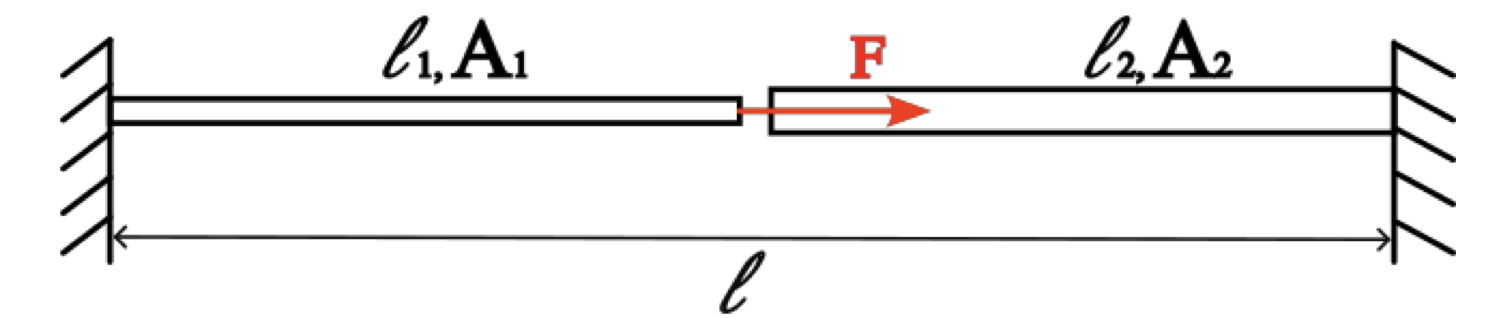
\includegraphics[width=0.6\linewidth]{media/merosA.png}
    \caption{Πρόβλημα πρώτου μέρους.}
    \label{fig:merosA}
\end{figure}

\par Στο δεύτερο μέρος διερευνάται η γραμμική και η σημειακή επαφή μέσω της θεωρίας του Hertz. Ζητείται η δημιουργία δύο μοντέλων για την επίλυση των δύο προβλημάτων. Για τη γραμμική επαφή, δημιουργείται μοντέλο ΠΣ δύο κυλίνδρων σε επαφή. Η δύναμη ασκείται στον έναν κύλινδρο και αναπτύσσονται έτσι οι τάσεις επαφών. Για τη σημειακή επαφή μελετάται η περίπτωση επαφής σφαίρας με επίπεδο. Τα προβλήματα αυτά θα επιλυθούν τόσο με αδρό πλέγμα όσο και με πυκνό. Οι επιλύσεις θα συγκριθούν με τα θεωρητικά αποτελέσματα από τη θεωρία του Hertz. Τα ζητούμενα είναι η αναπτυσσόμενη πίεση και το πλάτος επαφής, οι αναπτυσσόμενες κύριες τάσεις, η σχέση δύναμης-μετατόπισης.
\begin{figure}[H]
    \centering
    \begin{subfigure}{0.49\linewidth}
        \centering
        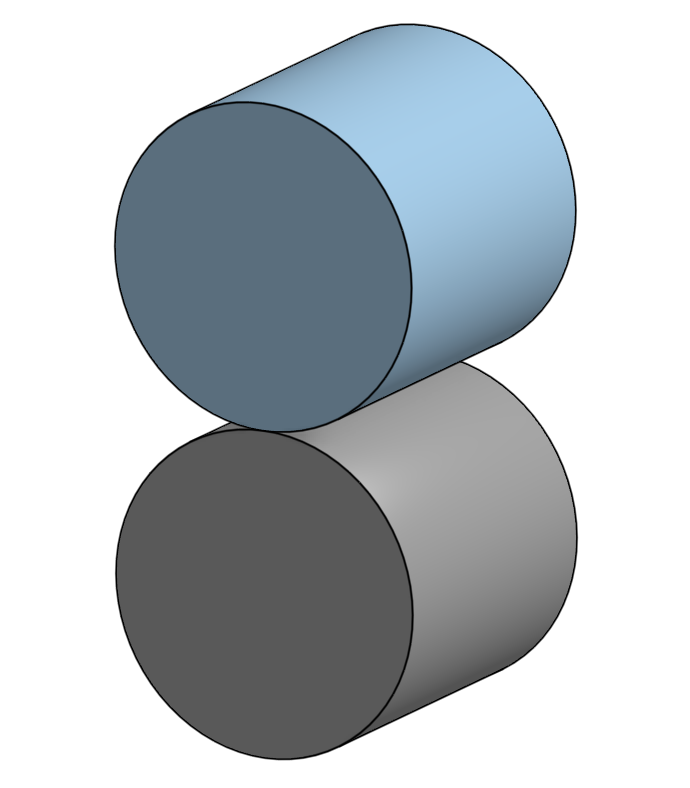
\includegraphics[width=0.6\linewidth]{media/kyl.png}
        \caption{Πρόβλημα γραμμικής επαφής.}
    \end{subfigure}
    \hfill
    \begin{subfigure}{0.49\linewidth}
        \centering
        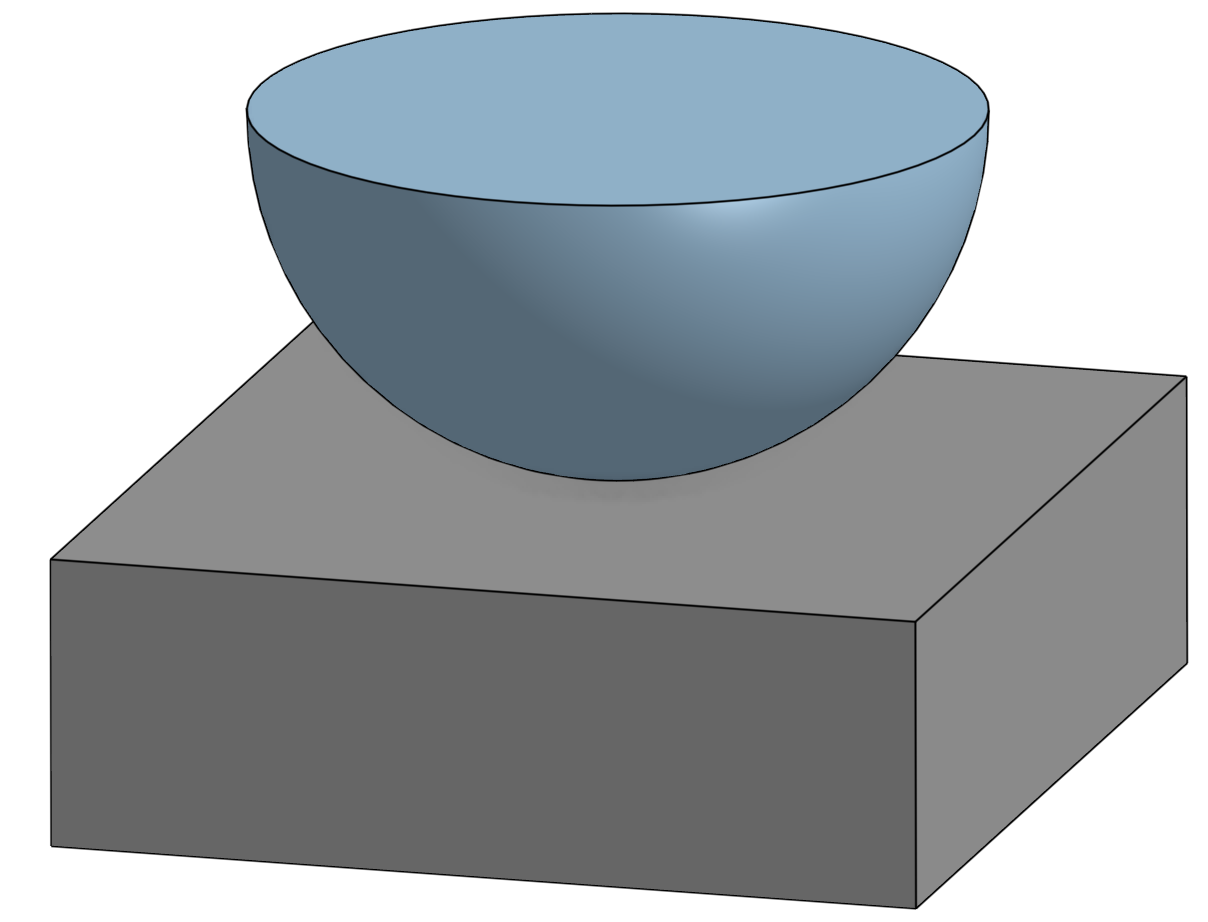
\includegraphics[width=0.6\linewidth]{media/sfaira.png}
        \caption{Πρόβλημα σημειακής επαφής.}
    \end{subfigure}
    \caption{Προβλήματα δεύτερου μέρους.}
    \label{fig:merosB}
\end{figure}



\subsection{Συνοπτική θεωρία}
\subsubsection{Μέθοδος ποινής}
Σύμφωνα με τη μέθοδο της ποινής, αφού τα σώματα έρθουν σε επαφή, ξεκινάει να δρα ένα ελατήριο με πολύ μεγάλη στιβαρότητα στον κόμβο της επαφής. Η σταθερά του ελατηρίου αυτού είναι $\epsilon >> k$. Έτσι, εισάγεται ένα νέο δυναμικό στο ισοζύγιο ενέργειας, αυτό του ελατηρίου με στιβαρότητα $\epsilon$. Πλέον, το πρόβλημα προς ελαχιστοποίηση είναι το:
 \begin{align}
    &\Pi_p = \frac{1}{2}Ku^2 - F u + \frac{1}{2}E g ^2\\
    &\text{s.t.}\;  g\cdot N = 0\\
\end{align}

Με τους πίνακες του συστήματος $K, u, F$ να είναι:
\begin{equation}
    K = \begin{bmatrix}
        k_1 &-k_1 & 0 & 0\\
        -k_1 & k_1 & 0 & 0\\
        0 &0 & k_2 & -k_2\\
        0 &0 & -k_2 & k_2\\
    \end{bmatrix},\; \vec{u} = \begin{pmatrix}
        0\\ u_1 \\ 0\\ 0
    \end{pmatrix},\; \vec{F} = \begin{pmatrix}
        0\\ F\\ 0\\0
    \end{pmatrix}, \; E = \begin{bmatrix}
        \epsilon & 0 & 0 & 0\\
        0 & \epsilon & 0 & 0\\
         0 & 0 & \epsilon & 0\\
         0 & 0 & 0 & \epsilon\\
    \end{bmatrix}, \vec{g} = l - l_1 - l_2 - \vec{u}
\end{equation}

Όπου $N$, η δύναμη επαφής η οποία υπολογίζεται ως:
\begin{equation}
    N = -\epsilon \cdot g
\end{equation}

Τελικά το πρόβλημα καταλήγει στην εξίσωση:
\begin{align}
    K\vec{u} - \vec{F} - E\vec{g} = 0 & <=>\\
    K\vec{u} - \vec{F} - E(l - l_1 - l_2 - \vec{u}) = 0&
\end{align}

Με έναν απλό μετασχηματισμό καταλήγουμε στην εξίσωση προς επίλυση του προβλήματος της επαφής:
\begin{equation}
    (E^{-1} K + I)\cdot \vec{u} = E^{-1}\cdot \vec{F}
\end{equation}

\begin{figure}[H]
    \centering
    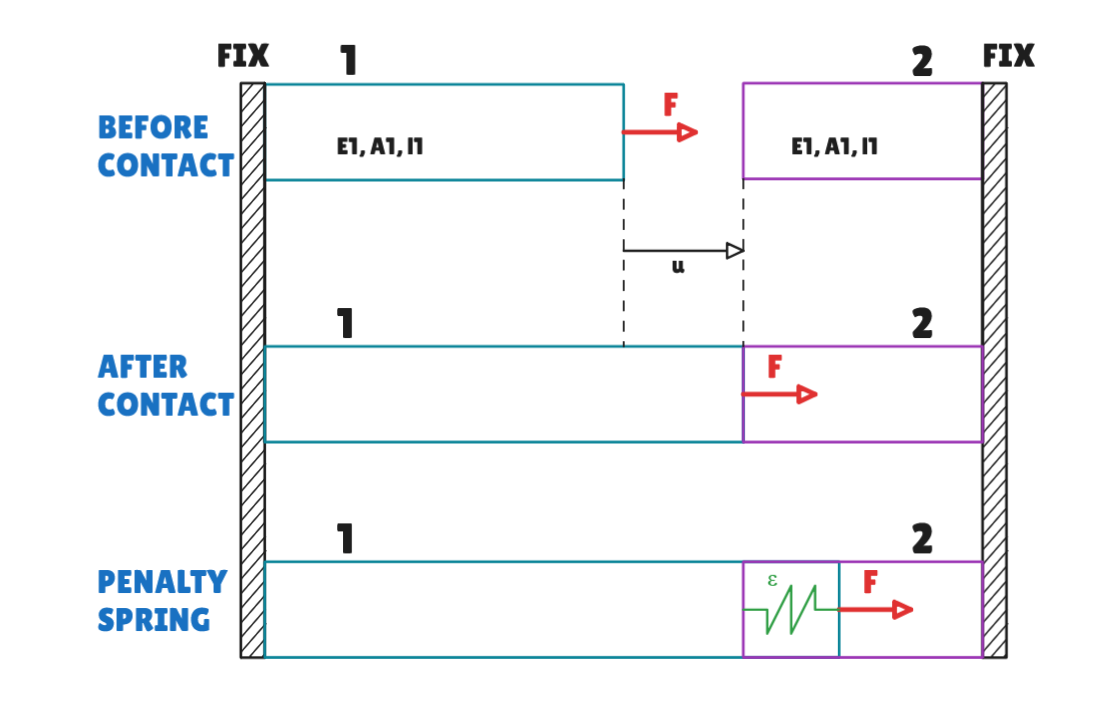
\includegraphics[width=0.6\linewidth]{media/pen.png}
    \caption{Μέθοδος ποινής.}
    \label{fig:pen}
\end{figure}



\subsubsection{Θεωρία Hertz}
Η γραμμική θεωρία του Hertz αναφέρει ότι, κατά την επαφή δημιουργείται ημιπλάτος επαφής που υπολογίζεται ως:
\begin{equation}
    \alpha = \sqrt{\frac{4 F R^*}{\pi E^* l}}
\end{equation}
Με τα ισοδύναμα μεγέθη $Ε^*$, $R^*$, για επαφή δύο κυλίνδρων $R_1, E_1, l$ και $R_2, E_2, l$ να υπολογίζονται ως:
\begin{align}
    \frac{1}{E^*} & = \frac{1-\nu_1^2}{E_1} + \frac{1-\nu_2^2}{E_2} \\
    \frac{1}{R^*} &= \frac{1}{R_1} + \frac{1}{R_2} 
\end{align}

Η πίεση επαφής κατά την διεύθυνση της επαφής δίνεται ως:
\begin{equation}
    p = \frac{2F}{\pi \alpha l} \sqrt{1 - \bigg(\frac{x}{\alpha}\bigg)^2} = p_0\sqrt{1 - \bigg(\frac{x}{\alpha}\bigg)^2}
\end{equation}


Η σχέση δύναμης μετατόπισης είναι γραμμική και δίνεται ως:
\begin{equation}
    F = \frac{\pi}{4}E^* l u
\end{equation}

Τέλος, οι κύριες τάσεις συναρτήσει του βάθους στον κύλινδρο δίνονται ως:
\begin{align}
    \sigma_x &= -2\nu p_0 \bigg(\sqrt{1 + \bigg(\frac{z}{\alpha}\bigg)^2} - \bigg|\frac{z}{\alpha}\bigg|\bigg)\\

    \sigma_y &= - p_0 \Bigg(\frac{1+2\frac{z^2}{\alpha^2}}{\sqrt{1 + \bigg(\frac{z}{\alpha}\bigg)^2}} - 2\bigg|\frac{z}{\alpha}\bigg|\Bigg)\\

    \sigma_z &= -\frac{p_0}{\sqrt{1 + \bigg(\frac{z}{\alpha}\bigg)^2}}
\end{align}



Αντίστοιχα, η θεωρία του Hertz για σημειακή επαφή, δηλαδή επαφή δύο σφαιρών,  αναφέρει ότι το πλάτος επαφής είναι:

\begin{equation}
    \alpha = \sqrt[3]{\frac{3 F R^*}{4 E^*}}
\end{equation}
Με τα ισοδύναμα μεγέθη $Ε^*$, $R^*$ να δίνονται με τον ίδιο τρόπο όπως στην επαφή των κυλίνδρων. Η πίεση επαφής κατά την ακτινική διεύθυνση δίνεται ως:
\begin{equation}
    p = \frac{3F}{2\pi \alpha^2} \sqrt{1 - \bigg(\frac{r}{\alpha}\bigg)^2} = p_0\sqrt{1 - \bigg(\frac{x}{\alpha}\bigg)^2}
\end{equation}

Στην περίπτωση επαφής σφαίρας δαπέδου απλώς ορίζεται ότι $R_2 = \inf$. Η σχέση δύναμης μετατόπισης δεν είναι γραμμική αυτή τη φορά και δίνεται ως:
\begin{equation}
    F = \frac{4}{3}E^* \sqrt{R^*} u^{3/2}
\end{equation}

Τέλος, οι κύριες τάσεις συναρτήσει του βάθους δίνονται ως:
\begin{align}
    \sigma_{x,y} &= - p_0 \bigg( \bigg(1-\bigg|\frac{z}{\alpha}\bigg| atan\bigg(\frac{1}{|z/\alpha|}\bigg)\bigg)(1+\nu)  - \frac{1}{2 (1 + \bigg(\frac{z}{\alpha}\bigg)^2)} \bigg)\\

    \sigma_z &= -\frac{p_0}{1 + \bigg(\frac{z}{\alpha}\bigg)^2}
\end{align}

\section{Μοντελοποίηση}

\subsection{Μέρος Α'}















\end{document}